\pdfoutput=1   % arXiv: force pdfLaTeX (we ship PNG figures); must sit in the first ~5 lines
% =====================================================================
%  Slide-Examiner technical report
%  Build:  pdflatex main && pdflatex main   (no bibtex; manual thebibliography)
%  Figures live in ./figs/ (PNG). Requires a full TeX Live (newtx, booktabs, ...).
%  Citations: all arXiv ids verified 2026-06-22 (see thebibliography). Author block is final pending the author's eyeball.
% =====================================================================
\documentclass[10pt]{article}

\usepackage[T1]{fontenc}
\usepackage[utf8]{inputenc}
\usepackage{amsmath}
\usepackage{amssymb}
\usepackage{newtxtext,newtxmath}     % Times-like, ML-paper look (load after ams*)
\usepackage[margin=1in]{geometry}
\usepackage{microtype}
\usepackage{graphicx}
\usepackage{booktabs}
\usepackage{array}
\usepackage{multirow}
\usepackage[table]{xcolor}    % [table] -> colortbl, enables \columncolor in the reward table
\definecolor{NavyBlue}{RGB}{31,90,135}
\definecolor{Accent}{RGB}{31,111,139}
\usepackage[font=small,labelfont=bf,skip=4pt]{caption}
\usepackage{subcaption}
\usepackage[percent]{overpic}    % text overlays on vector base art (concept figures)
\definecolor{figink}{HTML}{2B3440}
\definecolor{figslate}{HTML}{5A6675}
\definecolor{figblue}{HTML}{3F6FB5}
\definecolor{figorange}{HTML}{E07F2C}
\definecolor{figred}{HTML}{D24A43}
\definecolor{figgreen}{HTML}{4E9A6B}
\definecolor{figgrey}{HTML}{9AA4B0}
\usepackage{enumitem}
\usepackage[colorlinks=true,linkcolor=NavyBlue,citecolor=NavyBlue,urlcolor=NavyBlue]{hyperref}

\newcommand{\ba}{\textsc{bal-acc}}
\newcommand{\g}[1]{\textsf{#1}}        % defect-class names
\newcommand{\best}[1]{\textbf{#1}}
\newcommand{\ci}[1]{\,{\scriptsize[#1]}}   % compact 95% Wilson interval subscript
\setlist{nosep,leftmargin=1.4em}

\title{\bf Diagnose Before You Inspect:\\[2pt]
Failure Attribution Prescribes a Deterministic\\ Symbolic--Neural Critic for Slides}

\author{Ruihan Su\thanks{Independent technical report. All experiments were run on a single
4$\times$RTX~3080 (20\,GB) workstation; weights, renders, and raw rollouts are not redistributed but
all analysis scripts and reports are released. Correspondence: \texttt{surh6@mail2.sysu.edu.cn}.}\\[3pt]
\normalsize Sun Yat-sen University}
\date{}

\begin{document}
\maketitle

\begin{abstract}
\noindent
Vision--language models (VLMs) routinely pass slides with visible defects. We ask which failure mechanism
prevents inspection, then test whether that diagnosis predicts the effective inspection method. A lossless
structured-geometry oracle separates sub-perceptual, format-suppressed, and reference-assisted failures.
The resulting correspondence is concrete: declared geometry and terminology call for symbolic linting;
format-suppressed render overflow calls for an atomic, evidence-bearing VLM query; defects available only by
comparison call for a clean reference; and page semantics benefit from a finetuned examiner. On three vendors,
atomic elicitation beats a 10-sample compute-matched baseline by .20--.31 balanced accuracy while using one call.
We compose these methods deterministically, without a learned assignment model. The critic reaches .957 macro
balanced accuracy on held-out validation (nine classes, 150 positive and 150 clean examples each). A later
frozen image-arm check scores .826 on a disjoint seed-controlled set (nine classes, 30+30 each), counting
unresolved clean-reference requests as misses. Failures on clean \g{S6} controls,
pixel-recovered structure, and real \textsc{SlideAudit} layouts delimit where the prescription transfers.
\end{abstract}

% =====================================================================
\section{Introduction}
% =====================================================================

An automatic critic that flags layout and content defects is now a load-bearing component of every slide- and
document-generation agent, and the default critic is a general-purpose VLM asked to grade a rendered slide.
These critics fail in a revealing way: shown a slide whose title visibly spills out of its box, a strong VLM
under a standard rubric prompt answers ``no defect.'' Whether this is a failure of
\emph{perception} (it cannot see the overflow) or of \emph{elicitation} (it sees, but the way we ask buries
the signal) is rarely asked, yet the answer decides whether the remedy is a larger model, a different prompt,
or a different tool entirely. We treat that question as the design problem and answer it empirically.

\begin{figure}[t]
\centering
\begin{overpic}[width=\linewidth,percent]{figs/fig_teaser_notext.pdf}%
  \put(14.17,24.33){\makebox(0,0)[b]{\footnotesize\color{figslate} input slide}}
  \put(35.83,33.25){\makebox(0,0)[b]{\scriptsize\color{figink} perception /}}
  \put(35.83,31.58){\makebox(0,0)[b]{\scriptsize\color{figink} reasoning}}
  \put(35.83,30.08){\makebox(0,0)[b]{\scriptsize\bfseries\color{figink} diagnosis}}
  \put(57.08,43.25){\makebox(0,0)[b]{\footnotesize\bfseries\color{figblue} symbolic linter}}
  \put(57.08,41.42){\makebox(0,0)[b]{\scriptsize\color{figslate} declared geometry}}
  \put(57.08,9.08){\makebox(0,0)[b]{\footnotesize\bfseries\color{figorange} re-elicited VLM}}
  \put(57.08,7.25){\makebox(0,0)[b]{\scriptsize\color{figslate} format-suppressed}}
  \put(88.96,24.08){\makebox(0,0)[b]{\footnotesize\bfseries\color{figink} hybrid critic}}
  \put(50.0,1.83){\makebox(0,0)[b]{\scriptsize\itshape\color{figslate} G7 render-overflow (legal box, overflowing pixels) is linter-blind by construction; only a rendered-quality read-out catches it}}
\end{overpic}
\caption{\textbf{The paper in one picture.} A perception/reasoning diagnosis (Sec.~\ref{sec:diag}) shows
slide-inspection failures are of two kinds. Declared-geometry defects are exact and cheap for a symbolic linter,
with a sub-threshold acuity tail nothing recovers; merely format-suppressed defects are recovered by a
vision--language model under a changed elicitation. The diagnosed bottleneck deterministically selects the
inspection method, yielding a hybrid critic (Sec.~\ref{sec:hybrid}). A constructed render-overflow class (legal declared box,
overflowing pixels) is the crux: invisible to the linter by construction, it is caught only by engines with a
rendered-quality read-out (a re-elicited VLM, a frontier VLM judge, or general perceptual reward models), not by
domain-labelled scorers, so its detection tracks perceptual capability rather than training domain
(Sec.~\ref{sec:g7}).}
\label{fig:teaser}
\end{figure}

A VLM that ``cannot see'' a slide defect is hiding several failures of opposite character, and separating them
is the whole problem. Some defects are \emph{sub-perceptual} (i.e., below the tested models' effective
threshold under this protocol): a three-pixel alignment offset or a one-point font mismatch sits below the
model's effective acuity, and no amount of prompting, scale, or resolution recovers it. Others are
\emph{format-suppressed}: the model can perceive them, but the conventional elicitation (``here is a slide and
a rubric; score every defect type in one pointwise pass'') buries the signal, while a targeted atomic query
with required evidence recovers it with the model and image frozen. A third slice is \emph{reference-assisted}:
the model resolves the defect once a clean twin is available, but not from a single slide alone. Conflating
these cases is why the field oscillates between ``VLMs are bad at layout'' and ``VLMs can judge slides''; both
hold, for different defects.

We make the split measurable with an attribution protocol built on a \emph{lossless structured-geometry
oracle}. Each slide carries an intermediate representation (IR) of element bounding boxes, text, and style; we
present the same paired (defective, clean) slides under four input modalities (image-only, structured-oracle,
VLM-caption, and image+oracle) crossed with detect/localize/repair tasks. Because the oracle is lossless
machine-readable structure rather than a model-written caption, the perception channel it isolates is
uncontaminated: a model that fails image-only but succeeds with the structured oracle is bottlenecked on
perception, not reasoning. This is the methodological difference from concurrent perception/reasoning
attribution that uses natural-language perception oracles, which re-inject the very perceptual error they try
to factor out.

The diagnosis, not an architectural preference, then prescribes the critic (Fig.~\ref{fig:teaser}): assign
each defect to the method that addresses its bottleneck. Sub-perceptual geometry goes to a symbolic linter that
reads coordinates and rules; text and structural semantics go to a language model; and the format-suppressed,
perceivable classes go to a VLM, but only under the changed elicitation the diagnosis shows recovers them. To
stress-test the design we construct an adversarial render-containment overflow class that is invisible
to the linter by construction (the declared box is legal; only the rendered pixels overflow) and that we find
is missed by a 3B document reward and an artistic-aesthetic head as well, while two general-multimodal
rewards, a perceptual-quality probe, and a closed frontier VLM-as-judge see it; its detection tracks
rendered-quality read-out capability rather than the training-domain label alone. We conjecture the same
declared-layout/rendered-pixel gap recurs in DOM/CSS, charts, and document layout, but do not test it here. The
full symbolic--neural critic is built for \emph{IR-owning generation agents}, where the declared structure the
linter relies on is available; for bare third-party pixels the deployable critic is the re-elicited VLM
alone (Sec.~\ref{sec:external}), and every coverage claim should be read within that scope.

\paragraph{Contributions.}
Our contributions form a chain. We introduce a perception/reasoning attribution protocol built on a
\emph{lossless} structured-geometry oracle (element boxes, text, and style, not a model-written caption that
re-injects perceptual error) that separates a VLM's quality-inspection failures into \emph{sub-perceptual},
\emph{format-suppressed}, and \emph{reference-assisted} slices, and reproduces on real CC-licensed layouts with
no human or self-annotation (Secs.~\ref{sec:diag},~\ref{sec:external}). Applied across the taxonomy, the
protocol yields the paper's central finding: targeted defect-specific elicitation recovers the detection that
the conventional pointwise rubric buries, while \g{G1}/\g{S6} remain a distinct reference-assisted case rather
than evidence that the single-slide prompt ``saw it all along'' (Sec.~\ref{sec:hybrid}). A compute-matched
control then shows atomic \g{G7} recovery is not extra test-time compute: C3 beats ten-draw self-consistency by
.20--.31 across three vendors while using one call. The diagnosis finally \emph{prescribes} a deterministic
symbolic--neural critic, without a learned assignment model. It reaches .957 on held-out validation; a later
frozen image-arm check scores .826 on a disjoint set, with unresolved reference requests counted as misses.
Clean-control errors, recovered-structure failure, and real-layout
transfer bound the claim (Secs.~\ref{sec:hybrid},~\ref{sec:external}).

% =====================================================================
\section{Related work}
% =====================================================================

\paragraph{The VLM perception bottleneck.}
A growing line of work argues that VLM failures on visually grounded tasks are dominated by perception rather
than reasoning, decomposing the bottleneck for chart understanding~\cite{chartbottleneck} or showing that
the needed visual information is present in the representation but unused~\cite{hiddeninplainsight}; \textsc{MMVP}~\cite{mmvp}
is the canonical demonstration that VLMs stumble on minimally-different image pairs humans solve trivially, and
its sub-perceptual acuity floor is what our title (``not the eyes'') echoes. We share
the perception-first stance but ask it of a different task family, \emph{quality inspection of generated
artifacts}, where the perception channel can be isolated exactly with structured geometry rather than
approximated by captions, and where the answer feeds a critic architecture rather than a benchmark.

\paragraph{Perception/reasoning attribution.}
Concurrent work separates perception from reasoning in abstract visual-reasoning benchmarks via
natural-language perception oracles~\cite{reasoningbench}. We share the goal but differ in kind: our oracle is a
\emph{lossless} structured representation rather than a lossy caption, a cleaner attribution boundary because a
caption re-injects the very perceptual error it is meant to factor out; our domain of generated documents
admits exact injected labels; and we close the loop from diagnosis to a deployed critic.
Layout-error-detection work~\cite{led} introduces distribution-grounded structural-error injection but for
\emph{document-layout-analysis predictions}, and notes that existing metrics cannot isolate whether
failures stem from recognition or reasoning, the gap our attribution protocol fills.

\paragraph{Relative vs.\ absolute judgement.}
Our finding that relative elicitation beats absolute scoring echoes work showing VLM judges can rank but
cannot reliably score~\cite{rankscore}; that result concerns a judge's \emph{output mode}, orthogonal to our
\emph{source of failure}, and we adopt it to motivate the pairwise and atomic-binary heads of our critic.
Comparative/relative elicitation is also known to recover discriminative signal that pointwise scoring
suppresses in LLM/VLM judges~\cite{comparative}, though the protocol choice is not bias-free and can itself
distort preferences~\cite{pairpoint}. Our contribution is not that effect but its \emph{defect-class boundary}: it
rescues text overflow (\g{G1}) and image/text contradiction (\g{S6}) yet not fine alignment (\g{G3}) or
terminology drift (\g{S3}), which is what turns the elicitation effect into a perception/format attribution
signal.

\paragraph{Slide generation, evaluation, and reward.}
Slide and poster generation with design feedback is an active area: AutoPresent~\cite{autopresent} treats
slide generation as tool-augmented program generation with iterative self-refinement, aesthetic-reward
systems~\cite{aeslides,evopresent} report that iterative VLM refinement helps gross layout damage but fails on
fine-grained aesthetics and is prone to reward hacking, and slide-evaluation studies~\cite{vlmslideeval} call
for calibrated critic-in-the-loop selection. These \emph{motivate} a composed critic rather than compete with it:
they observe the VLM's perceptual ceiling and work around it with rules, whereas we first \emph{diagnose} that
ceiling and show part of it is elicitation-recoverable. We probe real data with the human-annotated
\textsc{SlideAudit} set~\cite{slideaudit} and audit five published reward/perceptual scorers spanning document,
general-multimodal, and aesthetic categories plus a closed frontier VLM-as-judge (Sec.~\ref{sec:g7}). Training
specialist critics from paired data is an established recipe in natural images and code; defect injection adapts
it to rendered documents at zero annotation cost, and we use it as the semantic engine of the prescribed critic and
the perception/reasoning attribution it enables.

% =====================================================================
\section{Problem setup and defect taxonomy}\label{sec:setup}
% =====================================================================

\paragraph{Task and representation.}
The critic inspects a single rendered slide, optionally with its declared structure, and must \emph{flag and
localize} defects of a fixed set of types; a detection counts only when it fires on a defective slide and stays
silent on its matched clean twin. Every slide is an intermediate representation (IR) of typed elements with
bounding boxes, text, and style; we inject defects programmatically into the IR and render, yielding exact
labels and matched (defective, clean) pairs. The taxonomy (Table~\ref{tab:taxonomy}) has a \emph{geometry}
group \g{G1}--\g{G6}, a \emph{semantic} group \g{S1}--\g{S6}, and one constructed render class \g{G7}; it is
aligned to the expert-derived \textsc{SlideAudit} taxonomy~\cite{slideaudit} via a bidirectional map, and
results are reported in its canonical classes (Appendix~\ref{app:slideaudit-crosswalk}). We add \g{G7} because
it is the sharpest test of the linter's blind spot: the declared box is legal (inside the safe margin, no
overlap) but the rendered content overflows its container, so the defect exists \emph{only} in pixels. On real
agent-generated decks \g{G7} is common, affecting most slides of a Zenodo10K slice and over half of an
AutoPresent slice.\footnote{93-deck Zenodo10K slice: 81/93 decks affected (857/3167 legal boxes); 14-deck
AutoPresent slice: 8/14 decks (20/50 legal boxes).}

\begin{table}[t]
\centering
\small
\caption{Defect taxonomy. The geometry group is detected symbolically; the semantic group is the examiner's
domain; \g{G7} is constructed to be linter-blind. ``Channel'' is the engine the diagnosis assigns
(Sec.~\ref{sec:diag}--\ref{sec:hybrid}).}
\label{tab:taxonomy}
\begin{tabular}{@{}llll@{}}
\toprule
Group & Class & Description & Channel \\
\midrule
\multirow{6}{*}{Geometry} & \g{G1} text overflow & text exceeds its box & VLM (pairwise) + linter \\
 & \g{G2} element overlap & boxes intersect & linter \\
 & \g{G3} alignment offset & small mis-alignment & linter \\
 & \g{G4} font-size inconsistency & off-grid font size & linter \\
 & \g{G5} brand-color violation & off-palette color ($\Delta E$) & linter \\
 & \g{G6} margin violation & element past safe margin & linter \\
\midrule
\multirow{6}{*}{Semantic} & \g{S1} title/body mismatch & body contradicts title & VLM \\
 & \g{S2} narrative-order break & deck sections out of order & LLM \\
 & \g{S3} terminology inconsistency & term drift across deck & term linter \\
 & \g{S4} density violation & slide over/under-packed & LLM \\
 & \g{S5} missing logic section & dropped argument step & LLM \\
 & \g{S6} image/text contradiction & figure contradicts caption & VLM \\
\midrule
Render & \g{G7} containment overflow & legal box, rendered overflow & VLM (atomic-binary) \\
\bottomrule
\end{tabular}
\end{table}

\paragraph{Attribution modalities and metric.}
We present each paired sample under four modalities: \textbf{A} image-only; \textbf{B} the lossless structured
oracle; \textbf{B$'$} a fixed VLM-written caption; and \textbf{C} image+oracle, each crossed with
detect/localize/repair (Fig.~\ref{fig:modtask}).\footnote{The oracle's ground-truth markers are stripped by a single regression-tested
de-leaking view. B$'$ is a lossy-caption control, not a second oracle: because it is VLM-produced, B's advantage
for isolating declared structure is a property of the channel by design, not an empirical claim that captions
are always worse.} The attribution logic is operational: A-fail $\wedge$ B-succeed means the class becomes
solvable once the same information is made explicit as lossless structure, so we diagnose it as
\emph{perception-bottlenecked}; A-fail $\wedge$ B-fail means the class is unsolved even at the structured
interface and is assigned to a symbolic method. The headline metric throughout is \emph{balanced accuracy on paired
clean controls}, never recall alone, which a model can saturate by always flagging.

\begin{figure}[t]
\centering
\begin{overpic}[width=\linewidth,percent]{figs/fig_modality_task_notext.pdf}%
  \put(32.92,54.83){\makebox(0,0)[b]{\footnotesize\bfseries\color{figink} Detect}}
  \put(57.08,54.83){\makebox(0,0)[b]{\footnotesize\bfseries\color{figink} Localize}}
  \put(81.25,54.83){\makebox(0,0)[b]{\footnotesize\bfseries\color{figink} Repair}}
  \put(10.0,42.25){\makebox(0,0)[b]{\scriptsize\bfseries\color{figink} image-only}}
  \put(10.0,29.75){\makebox(0,0)[b]{\scriptsize\bfseries\color{figink} structured oracle}}
  \put(10.0,17.25){\makebox(0,0)[b]{\scriptsize\bfseries\color{figink} VLM-caption}}
  \put(10.0,4.75){\makebox(0,0)[b]{\scriptsize\bfseries\color{figink} image + oracle}}
\end{overpic}
\caption{\textbf{Attribution protocol.} Each paired (defective, clean) slide is presented under four input
modalities (image-only, the lossless structured oracle, a fixed VLM-caption control, and image+oracle) crossed
with detect/localize/repair. Comparing image-only against the structured oracle is what isolates a clean
perception/reasoning split (Sec.~\ref{sec:diag}).}
\label{fig:modtask}
\end{figure}

\paragraph{Two linters.}
A geometry linter detects \g{G1}--\g{G6} from coordinates and rules (brand color via CIELAB $\Delta E_{2000}$, not RGB
distance), at zero false positives on clean slides. A terminology linter handles \g{S3} from an occurrence
table plus near-duplicate clustering, image-free. Both are the ``detectors of record'' prescribed by the diagnosis.

% =====================================================================
\section{Diagnosis: two kinds of blindness}\label{sec:diag}
% =====================================================================

\paragraph{Pointwise image-only inspection floors fine geometry.}
Under pointwise image-only inspection, \g{G2}--\g{G6} sit at chance for 4B and 8B models, and a 30B model breaks
only the coarsest class (\g{G1} overflow). This pointwise floor is invariant to the things one would tune first:
swapping the vision encoder across \emph{five} families (SigLIP2, an LLM-based encoder, InternViT, a
native-resolution NaViT, and MoonViT) leaves every model at the random line, differing only in
abstain-vs-over-flag bias, and raising input resolution from 1536 to 2048 changes nothing. The lever is the
elicitation and the defect magnitude, not the encoder or the pixel budget (the next paragraph and
Fig.~\ref{fig:sat} show targeted/relative elicitation lifts supra-threshold alignment well above chance), so
the floor is a property of the \emph{pointwise} protocol, not a hard capability limit. Either way the right
detector for declared geometry is the symbolic linter: it reads the coordinates directly at balanced accuracy
0.75--1.0 with zero false positives, cheaper and exact where the IR is available, not because the VLM cannot
see the defect.

\paragraph{But some apparent perceptual failures are elicitation artifacts.}
The same pointwise image-only setting hides a second, opposite phenomenon. For \g{G1} text overflow and \g{S6}
image/text contradiction, pointwise balanced accuracy is 0.50, indistinguishable from the genuinely
sub-threshold tail, yet a two-alternative forced choice between the defective and clean slide jumps to
1.00 (Fig.~\ref{fig:rel}): the defect is perceivable, but the single-slide pointwise call does not
surface it. We therefore treat \g{G1}/\g{S6} as \emph{reference-assisted}: recovery needs the clean twin, not
just a renamed single-image question. \g{G3} alignment behaves differently, but only \emph{above a magnitude threshold}: sweeping the
injected offset as an internal contrast (one element shifted from its aligned sibling column, decidable from the
slide alone), the forced choice saturates to $1.00$ by $16$\,px ($0.83\%$ of slide width) while the
sub-threshold tail ($\le8$\,px) stays at chance even side by side (Fig.~\ref{fig:sat}). So fine alignment is not
a class-level capability floor: above threshold it is format-suppressed and recoverable, with
a sub-perceptual residue only in the small-offset tail. (\emph{How} the elicitation helps differs by
class, a named target versus a paired clean reference, which we decompose in Sec.~\ref{sec:elicit}.) The
connecting thread is a \emph{magnitude-gated} recoverable-versus-sub-perceptual boundary rather than a
clean geometric/semantic split, and \g{S3} terminology (below) remains the one defect no elicitation rescues.

On the rebuilt corpus we also now have a human spot-check on the actual pairs cited here, not just the earlier
diagnosis runs. Replacing only the stale legacy \g{G3}/\g{G5} samples and keeping the other 55 pairs fixed,
the v2 pass verifies every sampled defect as visible and every clean twin as clean (73/73, Wilson lower bound
0.95 for both), with source-structure faithfulness 55/55 on the auditable classes. The delta is exactly where
the re-operationalisation says it should be: \g{G3} shifts from 0/7 on the old external-reference sample to
8/8 on the corrected within-list misalignment sample, and \g{G5} from 0/7 to 10/10 on the corrected
within-list chromatic clash sample; the non-replaced 55 pairs are unchanged.

\begin{figure}[t]
\centering
\begin{overpic}[width=0.9\linewidth,percent]{figs/fig_rel_vs_abs_notext.pdf}%
  \put(25.42,43.33){\makebox(0,0)[b]{\small\bfseries\color{figink} absolute (pointwise)}}
  \put(25.42,36.67){\makebox(0,0){\large\bfseries\color{figslate} ?}}
  \put(25.42,7.67){\makebox(0,0)[b]{\scriptsize\itshape\color{figslate} score one slide alone $\rightarrow$ at chance for \g{G1}/\g{S6}}}
  \put(74.58,43.33){\makebox(0,0)[b]{\small\bfseries\color{figink} relative (forced choice)}}
  \put(74.58,7.67){\makebox(0,0)[b]{\scriptsize\itshape\color{figslate} compare a pair $\rightarrow$ recovers perfect detection}}
\end{overpic}
\caption{\textbf{Two elicitations, same model and images.} Pointwise (absolute) scoring inspects one slide in
isolation; the forced choice compares a pair. For \g{G1} and \g{S6}, changing absolute to relative is what
recovers detection; quantified in Fig.~\ref{fig:rel}.}
\label{fig:relconcept}
\end{figure}

\begin{figure}[t]
\centering
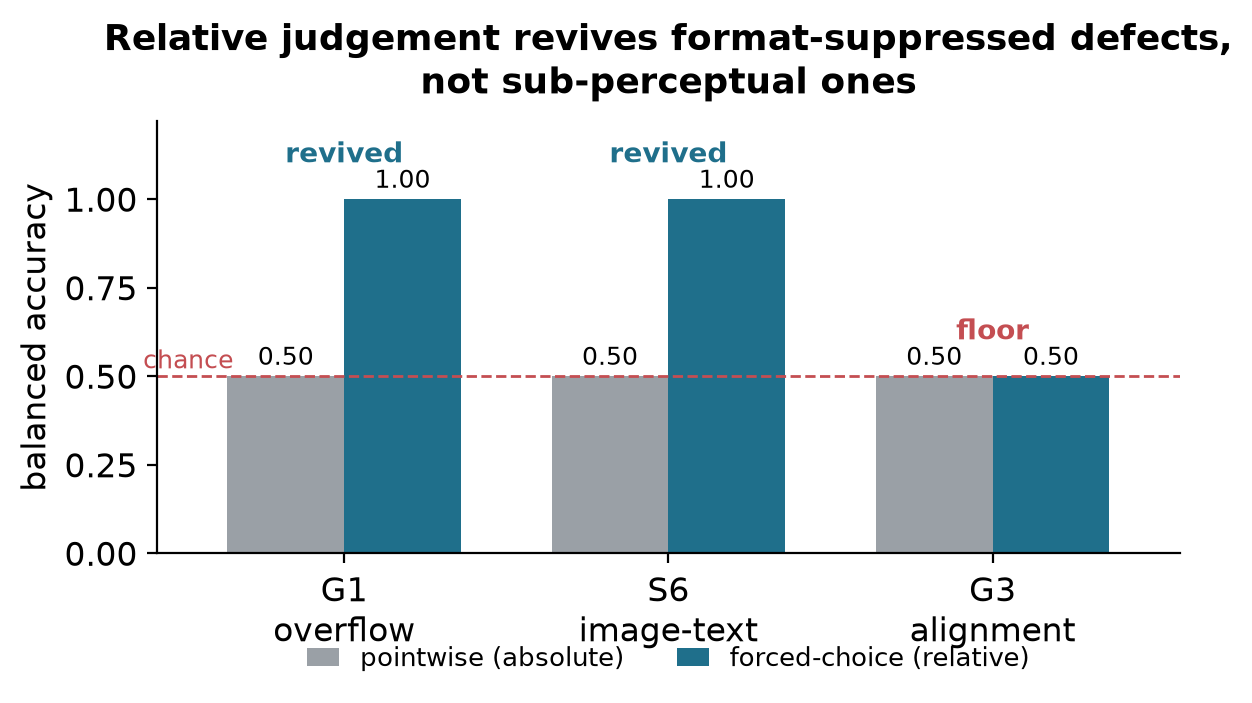
\includegraphics[width=0.72\linewidth]{figs/fig2_relative_vs_absolute.png}
\caption{\textbf{Relative judgement recovers absolute-pointwise blind spots.} For \g{G1} overflow and \g{S6}
image/text contradiction, pointwise (absolute) inspection is at chance but a forced choice recovers perfect
detection (\emph{elicitation-recoverable}). \g{G3} alignment behaves the same way above a magnitude threshold
(forced choice $1.00$ once the offset clears $\approx0.8\%$ of slide width; Fig.~\ref{fig:sat}); only its
sub-threshold tail and \g{S3} terminology stay at chance side by side. Same model, same images; only the
elicitation changes. What \emph{drives} the recovery (naming vs.\ a paired reference) is decomposed in
Fig.~\ref{fig:decomp}.}
\label{fig:rel}
\end{figure}

\begin{figure}[t]
\centering
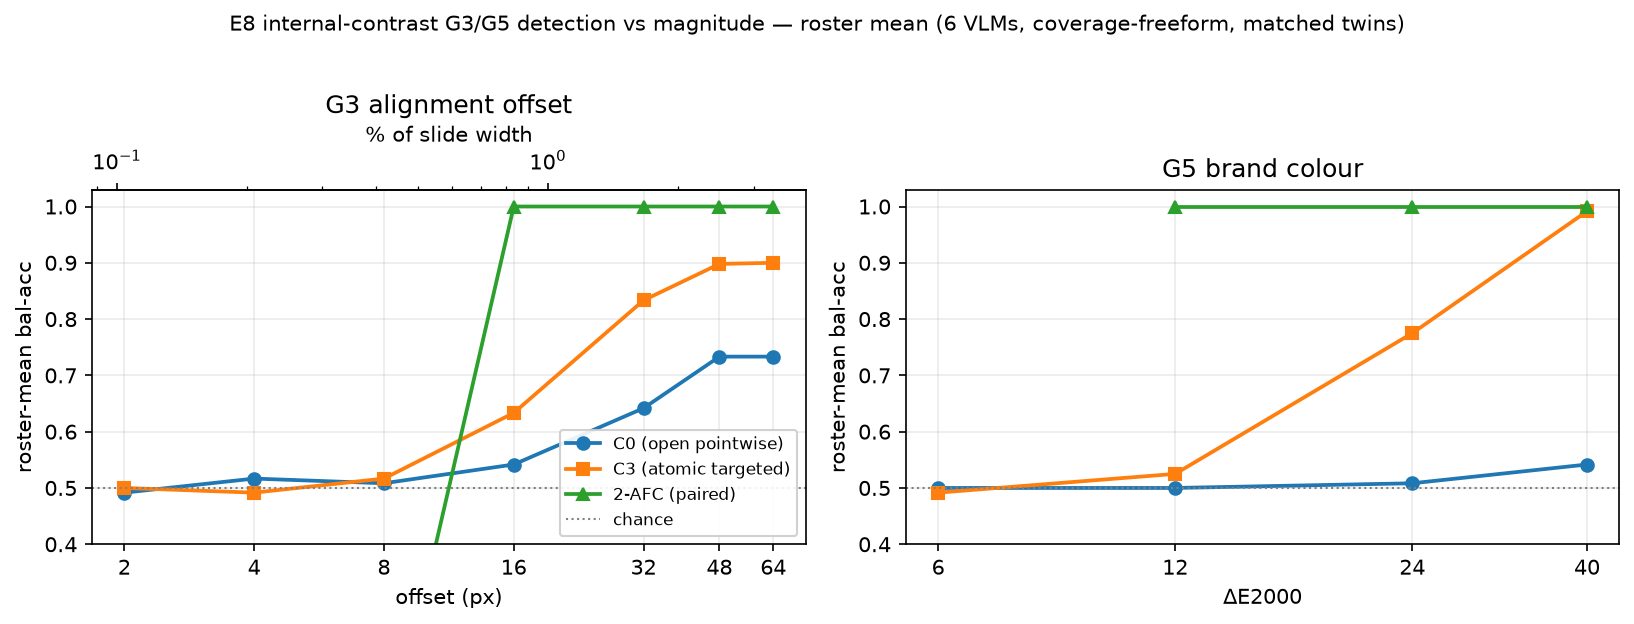
\includegraphics[width=\linewidth]{figs/fig10_g3_saturation.png}
\caption{\textbf{Fine geometry is magnitude-gated, not a flat capability floor.} Roster-mean balanced accuracy
(6 VLMs, matched-twin internal-contrast set) versus injected magnitude for \g{G3} alignment (left; px and \%
of slide width) and \g{G5} brand color (right; $\Delta E_{2000}$). Open pointwise (C0) lags; atomic targeted
elicitation (C3) recovers to a $\approx0.90$ plateau by $48$--$64$\,px / $0.99$ by $\Delta E\,40$; the paired
2-AFC saturates to $1.00$ by $16$\,px ($0.83\%$) / $\Delta E\,12$. The sub-threshold tail ($\le8$\,px,
$\le6\,\Delta E$) stays at chance under every protocol, the genuinely sub-perceptual residue. Single-slide C3
plateaus below $1.0$, a residual ceiling on \emph{absolute} spatial judgement that contrastive elicitation does
not share.}
\label{fig:sat}
\end{figure}

\paragraph{A counterexample: terminology.}
Not every consistency defect is format-suppressed. \g{S3} terminology inconsistency is \emph{not} rescued by
forced choice (0.625, heavy position bias): reading the same term across deck pages and spotting a subtle
variant is below threshold even side by side. The structured-oracle channel, which feeds the model
the full deck text with both variants present, also fails (0.56): with both variants already explicit in the
input, this failure cannot be OCR, and instead reflects cross-page term-matching that does not survive the
yes/no framing. The image channel is consistent with fine-grained glyph discrimination and the oracle channel
fails even with the text in hand, so neither neural method is reliable. \g{S3} leaves the VLM entirely for a symbolic terminology linter,
which reaches balanced accuracy 1.000 against the VLM's 0.69, a negative result that changes the prescribed method.

\paragraph{A genuine geometric blind spot: \g{G6} page offset.}
The re-operationalisation does not rescue every class; on one it fails outright. We re-pose \g{G6} margin as
a \emph{page offset}: the whole content block is shifted toward one edge (every element together, so internal
alignment is preserved and the defect cannot be misalignment), leaving one margin crowded against (or running
off) the edge and the opposite side empty, decidable from the slide alone.\footnote{The original \g{S6} render
omitted the figure element, so the cross-modal contradiction was literally unseeable (recall $0$); on the
valid-figure corpus the \g{S6} 2-AFC reproduces at $0.75$--$1.00$ across all six VLMs, confirming it is a
render artifact, not blindness.} Across all six VLMs and both pointwise framings (absolute ``past the safe
margin'' and relative ``shifted to one side'') the page offset stays at chance (roster-mean C3 $0.50$), and the
discriminative 2-AFC, the very test that separated \emph{data artifacts} (\g{S6} image/text contradiction,
which recovers to perfect once the figure is actually rendered) from genuine blindness, leaves \g{G6} on the
floor for \emph{every} model (Fig.~\ref{fig:artifact}): none can tell a page-offset slide from a balanced one
until the content is clipped by the page boundary. So unlike supra-threshold \g{G3}/\g{G5}
(format-suppressed) and \g{G1}/\g{S6} (reference-assisted), page offset is a \emph{genuine} perceptual blind spot (VLMs do not
represent global content positioning), which is why declared geometry is assigned to the linter.

\begin{figure}[t]
\centering
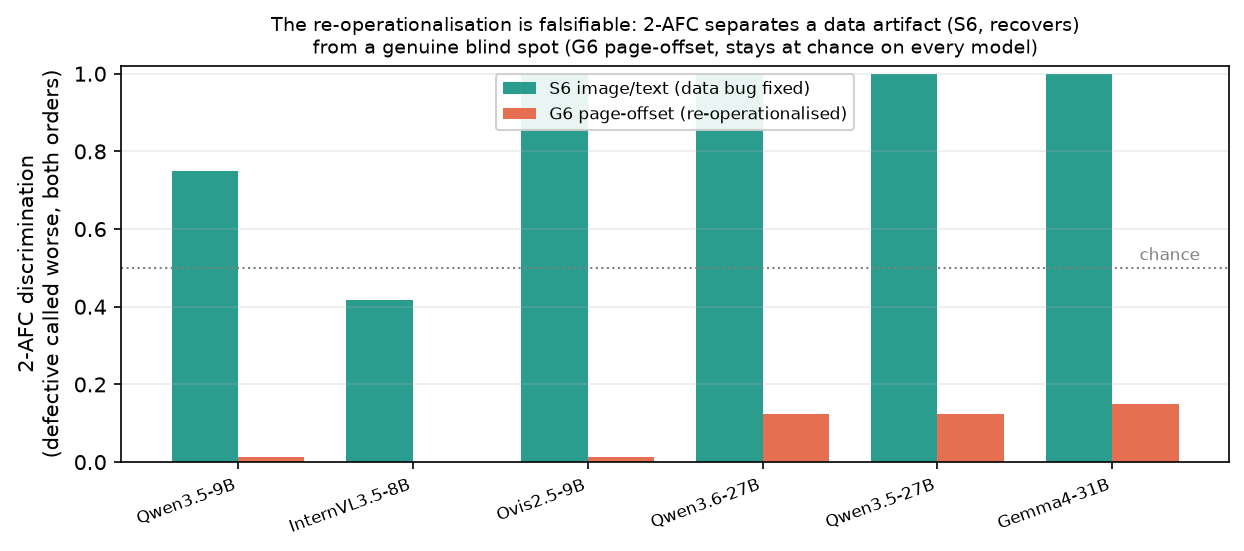
\includegraphics[width=0.92\linewidth]{figs/fig11_artifact_vs_genuine.png}
\caption{\textbf{A genuine blind spot the forced choice exposes.} Per-model 2-AFC discrimination (fraction of paired
slides where the defective is consistently called worse in both presentation orders; ties count as
not-discriminated). Single-image pointwise puts both classes at chance, but the forced choice \emph{separates}
them: the data artifact \g{S6} (image/text contradiction, on the fixed valid-figure corpus) recovers on every
model, while the re-operationalised \g{G6} page offset stays at the floor on every model: a genuine blind spot,
not an elicitation or data artifact.}
\label{fig:artifact}
\end{figure}

\paragraph{A methodological aside that becomes load-bearing.}
Enterprise ``snap-to-master'' templates re-fit element boxes to a grid before rendering, and we find a template
silently \emph{absorbs} 45\% of injected geometry defects: overlap, alignment, and margin violations become
pixel-identical to their clean twins after snapping, while overflow, driven by content-determined text
length, survives. This collapses the inspectable spectrum toward two poles, pure-perception defects templates
cannot constrain and pure-semantic defects they do not touch, and is a trap for any dataset that derives labels
from the IR but evaluates on the rendered image, a hazard we quantify and tie to a reward-model failure in
Sec.~\ref{sec:g7}.

% =====================================================================
\section{From diagnosis to a deterministic symbolic--neural critic}\label{sec:hybrid}
% =====================================================================

The diagnosis says a single model is the wrong unit. We prescribe a fixed correspondence from diagnosed failure
type to inspection method, validate the elicitation recovery across models, and stress the composition with the
constructed render class \g{G7}. This assignment is deterministic, not learned from class outcomes.

\subsection{Elicitation: format suppression is not capability}\label{sec:elicit}

\paragraph{Four ways to ask.}
We compare four elicitations holding the model and image fixed: \textbf{C0}, the conventional
pointwise+rubric pass over the whole taxonomy in one call; \textbf{C1}, free-form describe-then-classify;
\textbf{C2}, a geometry-normalized synthetic-twin pairwise (re-render snapped-to-grid, both orders); and
\textbf{C3}, an atomic per-type yes/no with forced localization. The scientific contrast is C3 vs.\ C0:
same model, taxonomy, and image, differing only in ``ask everything at once'' versus ``one atomic binary with
forced evidence.'' If C3 $\gg$ C0, the pointwise abstention was a format/cognitive-load artifact, not a
capability gap.

\paragraph{C3 recovers the linter-blind class across the capable subset.}
We scope the claim to models that can see \g{G7}: a model is in-scope only if C3 clears the
paired-clean detection gate ($\ba\ge0.70$, precision $\ge0.70$) and localizes the overflowing element, which
excludes InternVL-8B and Ovis-9B as capability-boundary cases. On the remaining four instances across three
scales and three vendors, atomic-binary C3 recovers detection that C0 suppresses (Fig.~\ref{fig:c3}:
$0.50$--$0.79\!\to\!0.93$--$1.00$, precision $0.88$--$1.00$). The effect we claim is \emph{cross-model}: a
stratified (Cochran) McNemar over the four models' matched pairs counts 233
\g{G7} items C3 fixes against 2 reversals ($\chi^2_1{=}227$, $p<10^{-50}$).\footnote{Per-model exact
McNemar $p\le1.5\!\times\!10^{-11}$, all Holm-surviving over the final paper-wide 85-test family; the two
reversals are on Gemma4-31B (C3 recall $88/90$). Full corrected table in the released multiplicity report.} The gate is defined by C3, but this cross-vendor test is gate-independent, so the recovery
is not a definitional artifact. The mechanism: C0's fixed whole-taxonomy rubric cannot \emph{name} an
off-taxonomy render class, so the model abstains; the atomic per-type binary restores it.

\begin{figure}[t]
\centering

\includegraphics[width=0.86\linewidth]{figs/fig5_c3_vs_c0_g7.png}
\caption{\textbf{Atomic-binary elicitation (C3) recovers the linter-blind render class \g{G7} across the capable
subset.}
Capable models reach the ceiling ($\ge$0.93, precision 0.88--1.0); the weaker InternVL/Ovis stay near their
perceptual floor, a capability-dependent boundary, not a universal fix.}
\label{fig:c3}
\end{figure}

\paragraph{It is the format, not the eyes.}
Does naming \g{G7} suffice, or does the \emph{atomic format} do the work? We separate them with a \textbf{C0+}
control (the C0 whole-taxonomy call with \g{G7} \emph{added} to the catalog, otherwise byte-identical) and a
single-slide \emph{C0\_named} condition that names the class on an isolated atomic prompt. The recovery factors
into coverage and format. \emph{Coverage}: naming recovers \emph{recall}, since C0$\to$C0+ flips 234
defectives from un-named to named against 0 reversals ($p{=}7\!\times\!10^{-71}$; named-recall
$0.00\!\to\!0.64$--$0.97$). \emph{Format}: but naming \emph{inside the overloaded rubric} wrecks
specificity, since C0+ over-flags clean twins on 55\% of pairs ($183/330$) versus 2.4\% ($8/330$)
for C3, so C0+ balanced accuracy stalls at $0.58$--$0.82$ while C3 reaches $0.93$--$1.00$. Naming the same class
on the \emph{atomic} prompt (C0\_named) instead recovers full balanced accuracy, and a paired clean reference
adds nothing on top (paired-clean Holm $p\le0.002$): so for \g{G7} the suppressor is the whole-taxonomy
\emph{format}, not a lack of visual signal. Forced evidence confirms real perception rather
than a lucky ``yes'': on the capable models' \g{G7} true positives the named region and overflowing element are
correct $\ge$98\%, and the models read back the specific spilling content (``the list items starting from `Cost
attribution'\,''), which a bluffing model cannot do. The same decomposition draws the boundary: for declared
geometry \g{G1} and image/text contradiction \g{S6}, naming alone does \emph{not} help (C0\_named
$\approx0.50$) and the recovery needs the paired reference (2-AFC $\to0.97$--$1.00$), a milder
\emph{reference-assisted} effect, not format suppression. A clean-vs-clean guess-floor rules out a
forced-pick artifact for both: capable models answer ``tie'' on $92$--$100\%$ of clean pairs
(Fig.~\ref{fig:decomp}).

\paragraph{Compute-matched control: recovery without additional test-time compute.}
The remaining alternative is that C3 wins only because it spends more test-time compute than the one-call rubric.
We test that directly on three API-served models spanning distinct vendors, holding the image and rendered corpus
fixed and matching C3's budget with repeated C0 draws. The headline control is \emph{self-consistency}: majority
vote over $K{=}10$ independent C0 samples. On \g{G7}, C3 still beats that compute-matched control on all three
vendors ($0.92/0.88/0.83$ vs. $0.61/0.59/0.63$; $\Delta{=}+0.31/+0.29/+0.20$), and all three contrasts survive
Holm correction within the full 24-test family (reported in the supplement). The budget points the same way:
C3 is the cheapest condition in completion tokens ($34.7/37.5/40.5$ output tok per slide, one call) while the
matched self-consistency baseline spends 8--10 calls per slide and still loses. The result is therefore not that a
heavier budget rescues the rubric; it is that the whole-taxonomy pointwise format suppresses detection, and breaking
that format recovers it without additional test-time compute. We report the union aggregation of the same draws, the
definition-matched one-call control, and the \g{G1} negative control in the supplement.

\begin{figure}[t]
\centering
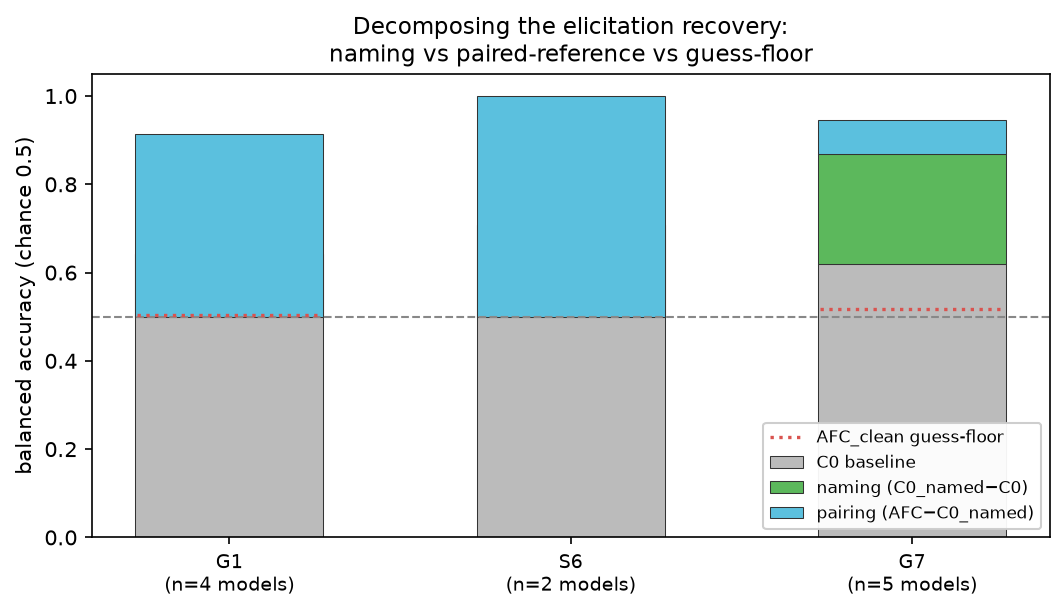
\includegraphics[width=0.78\linewidth]{figs/fig7_elicitation_decomp.png}
\caption{\textbf{What drives the recovery: naming vs.\ a paired reference.} Holding model and image fixed on the
freeform set, the chance$\to$ceiling jump factors into a \emph{naming} component (C0\_named$-$C0: one slide, the
defect named, \emph{no} reference) and a \emph{pairing} component (AFC$-$C0\_named: a clean twin supplied). For
the constructed render class \g{G7} the naming term carries it (green); for declared geometry \g{G1} and semantic
\g{S6} the paired reference does (blue). The AFC\_clean guess-floor (dotted) is near chance, so neither is a
forced-pick artifact. Mean over the models that recover ($\text{AFC}\ge0.7$).}
\label{fig:decomp}
\end{figure}

\paragraph{No universal elicitation, so the method must follow the diagnosis.}
The best elicitation is jointly set by model capability and defect class. C2 synthetic-twin pairwise (not
C3) rescues \emph{declared} geometry \g{G1} on capable models (Qwen3.5-27B $0.69\!\to\!0.93$, Qwen3.6-27B
$0.53\!\to\!0.78$, precision $1.00$), because snapping absorbs the declared overflow and the contrast exposes
it; and C1 free-form, which rescues weak abstaining models, \emph{collapses} on strong ones, which
free-associate nits and flag nearly every clean slide (precision $\approx0.50$). There is no one prompt, which
is why inspection must be assigned per diagnosed failure. The format effect is not a synthetic artifact: on the
human-annotated \textsc{SlideAudit} set, with no structure available, C3 still beats C0 for every class (brand
color $0.52\!\to\!0.81$, alignment $0.56\!\to\!0.72$). Absolute geometry on bare real pixels stays modest
($0.55$--$0.74$ outside blatant overlap): real fine geometry needs the linter, hence the element structure bare
images lack, so on image-only real data the hybrid runs in a degraded VLM-only mode, a ceiling set by missing
structure, not missing method.

\subsection{The minimal hybrid critic covers the most}\label{sec:coverage}

\paragraph{Complementary coverage the diagnosis predicts.}
On a novel-template held-out validation set with $150$ positives and $150$ clean controls per class, the
deterministic composition reaches .957 macro balanced accuracy (8/9 classes); \g{S6} is the sole miss because
97/150 clean controls fire. On a later disjoint seed-controlled set generated after the assignment was frozen,
with $30+30$ examples per class, the completed frozen image arm scores .8259 macro balanced accuracy and .7778
named localization, with unresolved clean-reference requests counted as misses. The first number is held-out
validation whose results had already been inspected; the second is a separate frozen check, not a corpus rerun.
We evaluate five critics by \emph{named attribution}: the correct defect must be emitted on the defective slide
and not on its clean twin, and a class is ``covered'' when named-attribution balanced accuracy exceeds $0.75$
(Wilson lower bound $>0.65$). Coverage follows what the diagnosis prescribes (declared geometry to the
linter, the format-suppressed classes to a C3-elicited VLM), and the headline is their \emph{combination}: the
linter alone covers 4/9 classes (mean bal-acc 0.66) and VLM-C3 alone 3/9 (0.72), but
\emph{linter $\oplus$ C3-VLM} covers 6/9 at 0.86, matching the prescribed composition
(6/9, 0.85), against the conventional VLM-C0's 1/9 (0.59) (Fig.~\ref{fig:coverage},
Table~\ref{tab:coverage}). The nine classes are the image-level paired-clean classes; \g{G4}/\g{S3} are
linter-owned and \g{S2}/\g{S5} are deck-scope (Sec.~\ref{sec:examiner}). A control settles why this is the
headline: per-class prompt/LLM tuning is \emph{not} load-bearing, since the assignment follows from the
diagnosis, not from optimizing over class outcomes, so the coverage is what the diagnosis predicts, not a tuned
architecture.

\begin{table}[t]
\centering\scriptsize
\setlength{\tabcolsep}{2pt}
\caption{Per-class named-attribution balanced accuracy with 95\% Wilson intervals; $n$ = paired positives with
matched clean controls (precision per cell in the released reports). The minimal linter+VLM-C3 hybrid matches
the prescribed coverage and slightly exceeds its mean. The small \g{S1} ($n{=}18$) and \g{S6} ($n{=}12$) cells are
method-selection diagnostics, not confirmatory tests: the \g{S6} reference-assisted and \g{S1} image-method
claims rest on the elicitation decomposition (Fig.~\ref{fig:decomp}) and the 2-AFC discrimination, not on these
cells.}
\label{tab:coverage}
\resizebox{\linewidth}{!}{%
\begin{tabular}{@{}llcccccr@{}}
\toprule
Class & method & linter & VLM-C0 & VLM-C3 & linter+C3 & prescribed & $n$ \\
\midrule
\g{G1} overflow      & linter & 1.00\ci{.91,1} & 0.50\ci{.46,.54} & 0.50\ci{.46,.54} & \best{1.00\ci{.91,1}} & \best{1.00\ci{.91,1}} & 40 \\
\g{G2} overlap       & linter & 0.80\ci{.68,.87} & 0.71\ci{.60,.79} & \best{0.86\ci{.74,.92}} & 0.80\ci{.68,.87} & 0.80\ci{.68,.87} & 40 \\
\g{G3} alignment     & linter & 0.93\ci{.85,.96} & 0.62\ci{.55,.68} & 0.71\ci{.63,.77} & \best{0.93\ci{.85,.96}} & \best{0.93\ci{.85,.96}} & 70 \\
\g{G5} color         & linter & 1.00\ci{.91,1} & 0.50\ci{.46,.54} & 0.68\ci{.57,.75} & \best{1.00\ci{.91,1}} & \best{1.00\ci{.91,1}} & 40 \\
\g{G6} margin        & linter & 0.75\ci{.67,.80} & 0.51\ci{.40,.61} & 0.51\ci{.47,.55} & \best{0.75\ci{.67,.80}} & \best{0.75\ci{.67,.80}} & 80 \\
\g{G7} render-overflow & VLM (C3) & 0.00\ci{0,.54} & 0.50\ci{.46,.54} & \best{1.00\ci{.91,1}} & \best{1.00\ci{.91,1}} & \best{1.00\ci{.91,1}} & 40 \\
\g{S1} title/body    & VLM (C0) & 0.50\ci{.41,.59} & \best{0.94\ci{.75,.98}} & 0.83\ci{.63,.92} & 0.83\ci{.63,.92} & \best{0.94\ci{.75,.98}} & 18 \\
\g{S4} density       & LLM & 0.50\ci{.45,.55} & 0.51\ci{.44,.59} & \best{0.93\ci{.81,.97}} & \best{0.93\ci{.81,.97}} & 0.72\ci{.60,.80} & 36 \\
\g{S6} image/text    & VLM & 0.50\ci{.38,.62} & 0.50\ci{.38,.62} & 0.50\ci{.38,.62} & 0.50\ci{.38,.62} & 0.50\ci{.38,.62} & 12 \\
\midrule
\multicolumn{2}{@{}l}{mean / classes covered} & 0.66 \,/\, 4/9 & 0.59 \,/\, 1/9 & 0.72 \,/\, 3/9 & \best{0.86 \,/\, 6/9} & 0.85 \,/\, 6/9 & \\
\bottomrule
\end{tabular}
}
\end{table}

\begin{figure}[t]
\centering

\includegraphics[width=0.86\linewidth]{figs/fig3_coverage_heatmap.png}
\caption{\textbf{Coverage by engine.} Per-defect balanced accuracy for the linter, VLM-C0, VLM-C3,
linter+VLM-C3, and the prescribed composition. Minimal linter$\oplus$C3 matches its coverage; \g{G7} (boxed) is the
linter-blind cell rescued by C3.}
\label{fig:coverage}
\end{figure}

\paragraph{A diagnostic method correction.}
We initially assigned \g{S1} title/body mismatch to the text LLM, but the text-only probe over-flags (0.25,
precision 0.09) while the image-bearing VLM names it reliably (0.94, precision 0.90): title/body mismatch needs
the \emph{rendered layout}, not just the text. We instead assign \g{S1} to the VLM under its \emph{open} pointwise
prompt (C0, 0.94) rather than the atomic C3 (0.83): recall is already saturated (both catch all 18 defectives),
so C3's forced yes/no only adds false positives, dropping specificity $0.89\!\to\!0.67$, a concrete case of the
per-class method selection of Sec.~\ref{sec:elicit}. The one image-level class the deployable hybrid does not
cover is \g{S6} image/text contradiction, at $0.50$ single-image for every engine; the 2-AFC forced choice
(Fig.~\ref{fig:artifact}) shows the model \emph{does} perceive it (recall $1.0$, specificity $\sim0$,
over-asserting rather than missing), so this is a \emph{reference-assisted} effect: it needs the
paired clean twin (Fig.~\ref{fig:decomp}), not a blind spot, in pointed contrast to the genuine \g{G6} page
offset.

\subsection{\g{G7}: the linter-blind class that specialised rewards also miss}\label{sec:g7}

\paragraph{Construction and headline split.}
\g{G7} makes the linter's blind spot falsifiable: a declared box that is legal (in-margin, non-overlapping) but
whose rendered content overflows its container. The IR carries only legal short text; the overflow lives in the
renderer, so the linter and any structure-only model are blind by construction---a self-check confirms zero
findings on 90/90 defectives. Auditing five published scorers plus one frontier VLM judge on the same paired
slides gives a decisive same-backbone dissociation: CLIP-IQA detects \g{G7} (0.83, $[0.74,0.90]$), while the
LAION aesthetic head on the same CLIP-L/14 is at chance (0.57, $[0.46,0.66]$). Across the scorers tested,
\g{G7} therefore tracks a rendered-quality read-out rather than the training-domain label. The complete
per-scorer table and the instance-level DocReward caveat are retained in the submission supplement.

\begin{figure}[t]
\centering
\begin{overpic}[width=\linewidth,percent]{figs/fig_g7_overflow_notext.pdf}%
  \put(25.42,4.17){\makebox(0,0)[b]{\footnotesize\color{figink} rendered text fits the box}}
  \put(74.58,4.17){\makebox(0,0)[b]{\footnotesize\color{figink} rendered pixels overflow the box}}
  \put(50.0,2.5){\makebox(0,0)[b]{\scriptsize\itshape\color{figslate} the linter sees two identical, legal declared boxes; it is blind to the difference by construction}}
\end{overpic}
\caption{\textbf{\g{G7} render-overflow.} The declared box (dashed) is legal and \emph{identical} in both
slides; only the rendered pixels overflow on the right. The geometry linter and any structure-only model read
the same legal box in both, so they are blind to \g{G7} by construction; only an engine with a rendered-quality
read-out catches it.}
\label{fig:g7fig}
\end{figure}

% The following reward-audit detail is retained for the technical-report version; the submission carries the
% complete table in its supplement.
\paragraph{Technical-report audit detail.}
The natural rebuttal is ``just train a neural reward model'' or ``use the frontier VLM as the judge.'' We test
both directly by auditing five published reward/perceptual scorers plus one closed frontier VLM-as-judge
on the same paired slides: does each score the clean slide above its defective twin? The scorers span three
categories. \emph{Document reward}: DocReward~\cite{docreward} (Qwen2.5-VL-3B, Bradley--Terry head
over 117K paired documents). \emph{General-multimodal rewards on distinct backbones}:
Skywork-VL-Reward-7B~\cite{skyworkvl} (Qwen2.5-VL-7B value head) and
PickScore~\cite{pickscore} (CLIP-H/14 contrastive reward, 500K human choices).
\emph{Aesthetic/perceptual scorers}: LAION-Aesthetic~\cite{laionaes} (linear artistic-appeal head on
CLIP-L/14) and CLIP-IQA~\cite{clipiqa} (zero-shot ``Good/Bad photo'' quality probe on the same CLIP).
The judge is Qwen3.7-Max on DashScope (pointwise 0--100 visual/layout-quality score). Each
penalizes several in-taxonomy defects it can see (Table~\ref{tab:reward}), confirming
each is a functioning scorer, not a domain mismatch.

\paragraph{The \g{G7} split: perceptual capability, not the domain label.}
On \g{G7} the picture splits, but \emph{not} along the domain label. The cleanest dissociation is within one
backbone: CLIP-IQA detects \g{G7} (0.83, $[0.74,0.90]$, $n{=}90$), while the LAION aesthetic head on the same
CLIP-L/14 is at chance (0.57, $[0.46,0.66]$). The same visible overflow is detected by \emph{both}
general-multimodal rewards on distinct backbones (Skywork-VL 0.79, $[0.69,0.86]$, Holm $p{=}2\!\times\!10^{-6}$;
PickScore 0.71, $[0.61,0.80]$, $p{=}2.5\!\times\!10^{-3}$) and by Qwen3.7-Max as a pointwise VLM judge (1.00,
$[0.86,1.00]$, $n{=}24$); it is missed (CI spans 0.5) by the symbolic linter (0.00), the artistic-aesthetic
LAION head (0.57), and the document reward (DocReward 0.48, $[0.38,0.58]$). The full split is in
Table~\ref{tab:reward}. (Naming containment in
Skywork's prompt lifts \g{G7} to 0.87, reinforcement rather than rescue. On \g{G5} (re-operationalised as an
internal chromatic clash, visible from the slide alone) \emph{most} scorers react (0.65--0.78), as the
perceptual-capability reading predicts; the linter still owns \g{G5} at 1.00 by exactness and palette
knowledge, not because the clash is imperceptible.)

\paragraph{What the split implies.}
The DocReward miss is \emph{instance-level}, not categorical: with a single 3B model capacity and training
objective are confounded, and a larger or differently-trained document reward may well detect \g{G7}. The
supported claim is narrower and stronger: \g{G7} is visible to general rendered-quality read-outs but can be
\emph{suppressed} by a specialised read-out on the \emph{same} backbone, and it is the reward-side counterpart
of the C0$\to$C3 recovery: the perception is present; the read-out, like the prompt format, can bury it. The
hybrid thesis is unchanged: \g{G7} needs a perceptually-capable engine, whether prompted, judged, or
reward-headed. Elicitation stays load-bearing even for the frontier judge: its whole-taxonomy prompt cannot
\emph{name} the off-taxonomy class (C0 $0.50$) while C3 names and localizes it perfectly (1.00).

\begin{table}[t]
\centering\small
\caption{Multi-reward / VLM-judge audit: paired preference accuracy $P(r_{\text{clean}}>r_{\text{def}})$ per class
(chance $=0.5$; \g{G7} with 95\% CI). Five published scorers in two audited categories each (general-multimodal:
Skywork-VL + PickScore on distinct backbones; aesthetic: LAION + CLIP-IQA) plus one closed frontier VLM judge,
so the \g{G7} read is not a single-scorer anecdote. \checkmark/$\times$ marks reliable \g{G7} detection (CI above
/ spanning 0.5). The VLM-judge row is a small closed-model probe ($n{=}24$); other $n$ in the bottom row.
\g{G5} is the internal-chromatic re-operationalisation of Sec.~\ref{sec:diag} (one element hue-swapped vs.\ its
sibling column), a \emph{visible} defect most scorers catch, not the linter-only blind spot \g{G7} is.}
\label{tab:reward}
\begin{tabular}{@{}llccc>{\columncolor[gray]{0.92}}c cc@{}}
\toprule
Reward scorer & category & \g{G1} & \g{G2} & \g{G5} & \textbf{\g{G7}} & \g{S4} & \g{S6} \\
\midrule
DocReward-3B   & document   & 0.93 & 1.00 & 0.72 & $\times$\,\textbf{0.48}\,{\scriptsize$[.38,.58]$} & 1.00 & 1.00 \\
\midrule
Skywork-VL-7B  & general-mm & 0.94 & 0.72 & 0.57 & \checkmark\,\textbf{0.79}\,{\scriptsize$[.69,.86]$} & 0.92 & 1.00 \\
PickScore-v1   & general-mm & 0.74 & 0.59 & 0.70 & \checkmark\,\textbf{0.71}\,{\scriptsize$[.61,.80]$} & 1.00 & 0.72 \\
\midrule
LAION-Aesth.   & aesthetic  & 0.37 & 0.91 & 0.78 & $\times$\,\textbf{0.57}\,{\scriptsize$[.46,.66]$} & 0.75 & 0.61 \\
CLIP-IQA       & aesthetic  & 0.44 & 0.50 & 0.65 & \checkmark\,\textbf{0.83}\,{\scriptsize$[.74,.90]$} & 0.50 & 0.72 \\
\midrule
Qwen3.7-Max judge & frontier VLM & 0.13 & 0.92 & -- & \checkmark\,\textbf{1.00}\,{\scriptsize$[.86,1]$} & 1.00 & -- \\
\midrule
\multicolumn{2}{@{}l}{$n$ (paired; non-VLM rows)} & 54 & 54 & 80 & 90 & 36 & 18 \\
\multicolumn{2}{@{}l}{$n$ (Qwen3.7-Max judge row)} & 24 & 24 & -- & 24 & 24 & -- \\
\bottomrule
\end{tabular}
\end{table}

\paragraph{Perturbation fidelity: 45\% of injected geometry never renders.}
The reward audit ties to the template result of Sec.~\ref{sec:diag}. Rendering every injected defective two
ways (faithfully and snapped-to-master), we find 45\% of injected geometry defects (100\% of overlap,
alignment, margin; 20\% of overflow) become pixel-identical to their clean twin after snapping. Feeding the
\emph{snapped} pairs to \emph{all five} reward scorers gives preference accuracy 0.00 at a reward gap of exactly
0.000: the two images are pixel-identical, so no critic (document, general-multimodal, or aesthetic) can react, a
dataset-integrity hazard (identical inputs force identical scores), not a reward-model deficiency.
This part \emph{is} model-agnostic by construction, and any reward model trained or evaluated on snap-rendered
images with IR-derived labels inherits these zero-signal pairs. Perturbation fidelity must be checked at the pixel
level, not assumed from the IR, a prerequisite the field largely skips, and the reason our elicitation
experiments render defectives faithfully.

% =====================================================================
\section{The semantic engine: a specialist examiner}\label{sec:examiner}
% =====================================================================

The hybrid's semantic engine can be a zero-shot model, but a small specialist does better on its own ground. We
finetune Qwen3-VL-8B with QLoRA on 2{,}142 injected supervision records; the submission supplement summarizes
the training mix and full evaluation table.

\paragraph{An 8B examiner surpasses a zero-shot 30B on \emph{in-distribution} semantics.}
On in-domain held-out page-semantic inspection, the finetuned 8B reaches balanced accuracy 1.000 on both
\g{S1} title/body and \g{S4} density, beating both zero-shot baselines including the 30B (0.93 / 0.77).
The largest gap is \g{S4} density (1.00 vs.\ 0.77 for the 30B), and both in-distribution contrasts survive
Holm correction over the final 85-test family. Thus, on the examiner's native in-distribution semantic tasks, the
specialist 8B beats the larger zero-shot model; full format-control and severity results are in the supplement.

\begin{table}[t]
\centering\small
\caption{Page-semantic inspection, balanced accuracy [95\% Wilson] on paired clean (best modality). The
finetuned 8B examiner beats both zero-shot baselines, including the 30B, \emph{in-distribution}. Deck-scope
\g{S2}/\g{S5} are a negative result (text). $n$ = paired positives (2-AFC rows = forced-choice pairs);
the \g{S6} 2-AFC rests on only 12 pairs and is descriptive only. ``Best modality'' denotes the
diagnostic-prescribed modality (oracle channel B for geometry, image-only for semantics), pre-determined by the
attribution logic, not selected post-hoc.}
\label{tab:examiner}
\begin{tabular}{@{}lcccr@{}}
\toprule
class & \textbf{ft-8B} & zs-8B & zs-30B & $n$ \\
\midrule
\g{S1} title/body  & \best{1.000}\ci{.95,1} & 0.778\ci{.69,.85} & 0.933\ci{.87,.95} & 36 \\
\g{S4} density     & \best{1.000}\ci{.97,1} & 0.529\ci{.50,.58} & 0.774\ci{.69,.84} & 60 \\
\g{G1} overflow (2-AFC) & \best{1.000}\ci{.97,1} & 0.975\ci{.93,.99} & 0.700\ci{.61,.77} & 120 \\
\g{S6} image/text (2-AFC) & \best{1.000}\ci{.76,1} & 1.000\ci{.76,1} & 0.500\ci{.25,.75} & 12 \\
\midrule
\g{S2} narrative (deck) & 0.500$^\dagger$\ci{.45,.53} & 0.646\ci{.53,.72} & 0.549\ci{.42,.66} & 36 \\
\g{S5} missing-logic (deck) & 0.500\ci{.47,.53} & 0.500\ci{.47,.53} & 0.567\ci{.45,.68} & 60 \\
\bottomrule
\end{tabular}
\\[2pt]
{\footnotesize $^\dagger$ degenerate (always-flag): the SFT mix had no clean-\emph{deck} negatives. See text.}
\end{table}

\paragraph{It abstains instead of hallucinating geometry.}
Under image-only inspection, the finetuned model stays at 0.50 on \g{G2}--\g{G6} with \emph{zero} false
positives: trained with image-only abstention targets, it declines to hallucinate geometry from pixels and
leaves those classes to the linter, the designed behavior, and the reason the hybrid's geometry column comes
from the linter rather than the VLM.

\paragraph{The main negative result is sim-to-real.}
The examiner does not transfer as a bare-pixel real-world inspector. On image-only \textsc{SlideAudit}, its
synthetic \g{S4} strength collapses to chance (0.50), whereas only the zero-shot 30B shows real density signal
($p{=}1.1\!\times\!10^{-5}$). Scale, not finetuning, carries bare-pixel transfer: the examiner learned a
distribution, not universal slide quality.

% =====================================================================
\section{External validity}\label{sec:external}
% =====================================================================

\paragraph{A real pre-sales agent deck.}
We run the same five-level examiner gradient on a real 16-slide proposal produced by a deployed PowerPoint
agent. Its verifiable defect is 20 unfilled template placeholders (``add a title here'') across 7 of 16
slides, a semantic-completeness defect the geometry linter is blind to by construction (the boxes are
geometrically fine). The result reinforces the thesis from an unexpected angle: the zero-shot 30B is the best
detector (recall 1.0, names the placeholder on 4/7 slides, scores them 0.03 vs.\ 0.64 for clean), while the
\emph{finetuned} 8B, top of the intrinsic-quality ranking, is among the \emph{worst} on this out-of-distribution
defect (names it 0/7), and the linter's apparent recall is spurious geometry noise with zero placeholder
mentions. The ranking on a novel defect is by general-VLM ability, not by the specialist's in-distribution
quality: the examiner learned a distribution, not universal quality. Feeding the flagged placeholders back to
the agent's own generator for one revision pass drives the verifiable defect from 20 to 0.

\paragraph{The structured attribution holds on real layouts.}
The body runs the A/B/C attribution on synthetic slides; the cleanest discrimination needs it on \emph{real}
geometry with a \emph{real} oracle, which seemed to require human or model annotation. We obtain it without either:
\textsc{Zenodo10K}~\cite{zenodo10k} ships real CC-licensed \texttt{.pptx} with intact element XML, so
\texttt{python-pptx} extracts a geometry/text/style oracle \emph{lossless with respect to the declared IR}
straight from the source file (the IR$\to$render gap that \g{G7} exploits is exactly what this oracle does
\emph{not} capture, by design), with no human or self-annotation bias. From 26 real decks we inject one single-shape defect per slide
\emph{in PPTX XML space} (overflow, overlap, alignment offset, font, margin) and render both the clean and the
defective one-slide deck with the same real renderer (LibreOffice), so the paired pixel diff isolates the injected
defect on real pixels (209 paired slides, 5 classes, 3 VLMs / 3 families). Two results follow. First, the
\S\ref{sec:diag} ``snap absorbs 45\%'' hazard is \emph{template-specific}: real free-form decks absorb only
7\% (render-fidelity 0.93), so the perturbation is faithfully present, a positive control on that claim.
Second, \emph{all three} attribution outcomes appear on real geometry: coarse defects (overflow, overlap) are
image-sufficient (balanced accuracy A~$0.70$--$0.74$, structure adds nothing); a margin bleed is a
perception bottleneck the oracle rescues for the weaker VLMs (A~$0.59 \to$ B~$0.70$), the
``missing structure, not missing capability'' cell; and fine alignment stays near chance in \emph{every}
channel for \emph{every} model (A~$=$~B~$=$~C~$\approx 0.50$; the internal-contrast re-run at a supra-threshold
$44$\,px offset reproduces this, A~$0.54$/B~$0.51$/C~$0.52$, $n{=}41$). This is \emph{not} a hard capability
floor: on clean synthetic slides the same alignment defect recovers under targeted/relative elicitation once it
clears acuity (Fig.~\ref{fig:sat}); but on real cluttered layouts the misaligned element cannot be isolated
among many genuine ones and specificity collapses, so for declared geometry the symbolic linter (which reads the
coordinates) remains the reliable detector regardless (Fig.~\ref{fig:real}).

\begin{figure}[t]
\centering

\includegraphics[width=0.82\linewidth]{figs/fig6_real_attribution.png}
\caption{\textbf{The perception/capability split reproduces on real layouts} (\textsc{Zenodo10K} real renders +
lossless \texttt{python-pptx} oracle; mean over 3 VLMs / 3 families, balanced accuracy on paired clean; error
bars = 95\% Wilson on counts pooled across models, $n{=}76$--$90$ paired per class). Coarse
defects (\g{G1} overflow, \g{G2} overlap) are image-sufficient; \g{G6} margin is a \emph{perception} bottleneck the
structured oracle rescues (B${>}$A); \g{G3} alignment stays near chance in every channel on these real cluttered
decks (A${=}$B${=}$C${\approx}0.5$), not a hard capability floor (it recovers on clean slides above threshold,
Fig.~\ref{fig:sat}) but unreliable enough on real layouts that it must fall back to the linter. Intervals on
\g{G3}/\g{G4}/\g{G6} include chance, consistent with their small per-class $n$ (see released reports).}
\label{fig:real}
\end{figure}

\paragraph{Open-world: structure recovered from pixels does not restore the linter.}
The hybrid's symbolic engine needs the declared IR a \texttt{.pptx} carries; a third-party deck exported to
PDF/PNG ships none, so the natural question is whether \emph{recovering} element structure from the rendered
pixels can re-arm the linter. We test it: following the DocLayNet/PubLayNet line of document-layout
detection datasets and benchmarks~\cite{doclaynet,publaynet}, a transformers-native detector (PP-DocLayoutV2)
returns region boxes on each render, class-agnostic NMS removes the detector's cross-class duplicate boxes
(which would otherwise manufacture phantom overlaps), and the boxes, normalised into the IR coordinate
frame, feed the \emph{same} geometry linter at its shipped operating point. On the real-layout set
(GT IR \emph{and} render available, so the full ladder and a recovery-fidelity IoU coexist) the answer is a
pre-registered negative (Fig.~\ref{fig:openworld}): recovered structure leaves the linter at chance on
\g{G1}/\g{G3}/\g{G4} (overflow needs text capacity, alignment needs declared positions, font needs point
sizes, none surviving a pixel$\to$box projection), and rescues only overlap partially (\g{G2} balanced accuracy
$0.54$ vs.\ native-IR $0.67$ vs.\ VLM-only $0.87$). The detector \emph{over-segments} ($\approx2\times$ more
boxes than the GT IR, recovery recall at IoU${\geq}0.5$ only $0.30$--$0.39$), so genuine element collisions are
split apart and overlap recall falls $0.78\to0.29$. The same picture holds on image-only \textsc{SlideAudit}
(no IR at all): the recovered linter clears chance only on \g{G2} ($0.55$) while the C3-elicited VLM reaches
$0.94$. Two points sharpen the deployment scope. First, on real third-party decks even \emph{native} IR is
weakened: the decks carry no expected-position/font bookkeeping, so the linter's \g{G3}/\g{G4} rules are also at
chance, and its margin/overlap rules \emph{over-fire} on tight real layouts (specificity $0.11$/$0.56$), eroding
the near-zero-false-positive advantage it enjoys on clean synthetic IR. Second, as a consequence the
VLM-only engine \emph{dominates every coarse class} on real decks. The linter's edge is an in-distribution,
clean-native-IR phenomenon; open-world, recovered or not, the deployable critic is VLM-bound. This bounds the
contribution without touching the diagnostic thesis: the full symbolic--neural critic is for IR-owning generation
agents, and for bare third-party pixels the critic is the C3-elicited VLM.

\begin{figure}[t]
\centering
\begin{overpic}[width=\linewidth,percent]{figs/fig_openworld_notext.pdf}%
  \put(14.06,14.69){\makebox(0,0)[b]{\footnotesize\color{figslate} raw pixels (no IR)}}
  \put(34.77,17.34){\makebox(0,0)[b]{\footnotesize\color{figslate} layout parser}}
  \put(55.31,15.0){\makebox(0,0)[b]{\footnotesize\color{figslate} recovered structure}}
  \put(55.31,13.28){\makebox(0,0)[b]{\scriptsize\itshape\color{figgrey} (approximate, not native IR)}}
  \put(81.25,29.84){\makebox(0,0)[b]{\footnotesize\bfseries\color{figred} symbolic linter}}
  \put(81.25,28.12){\makebox(0,0)[b]{\scriptsize\itshape\color{figred} not restored}}
  \put(80.47,3.52){\makebox(0,0)[b]{\footnotesize\bfseries\color{figblue} re-elicited VLM}}
\end{overpic}
\caption{\textbf{Open world: recovered structure does not restore the linter.} For bare third-party pixels with
no IR, a layout parser recovers approximate structure, but it is not the native IR the symbolic linter needs;
only the re-elicited VLM remains a deployable critic (quantified in Fig.~\ref{fig:openworld}).}
\label{fig:openconcept}
\end{figure}

\begin{figure}[t]
\centering
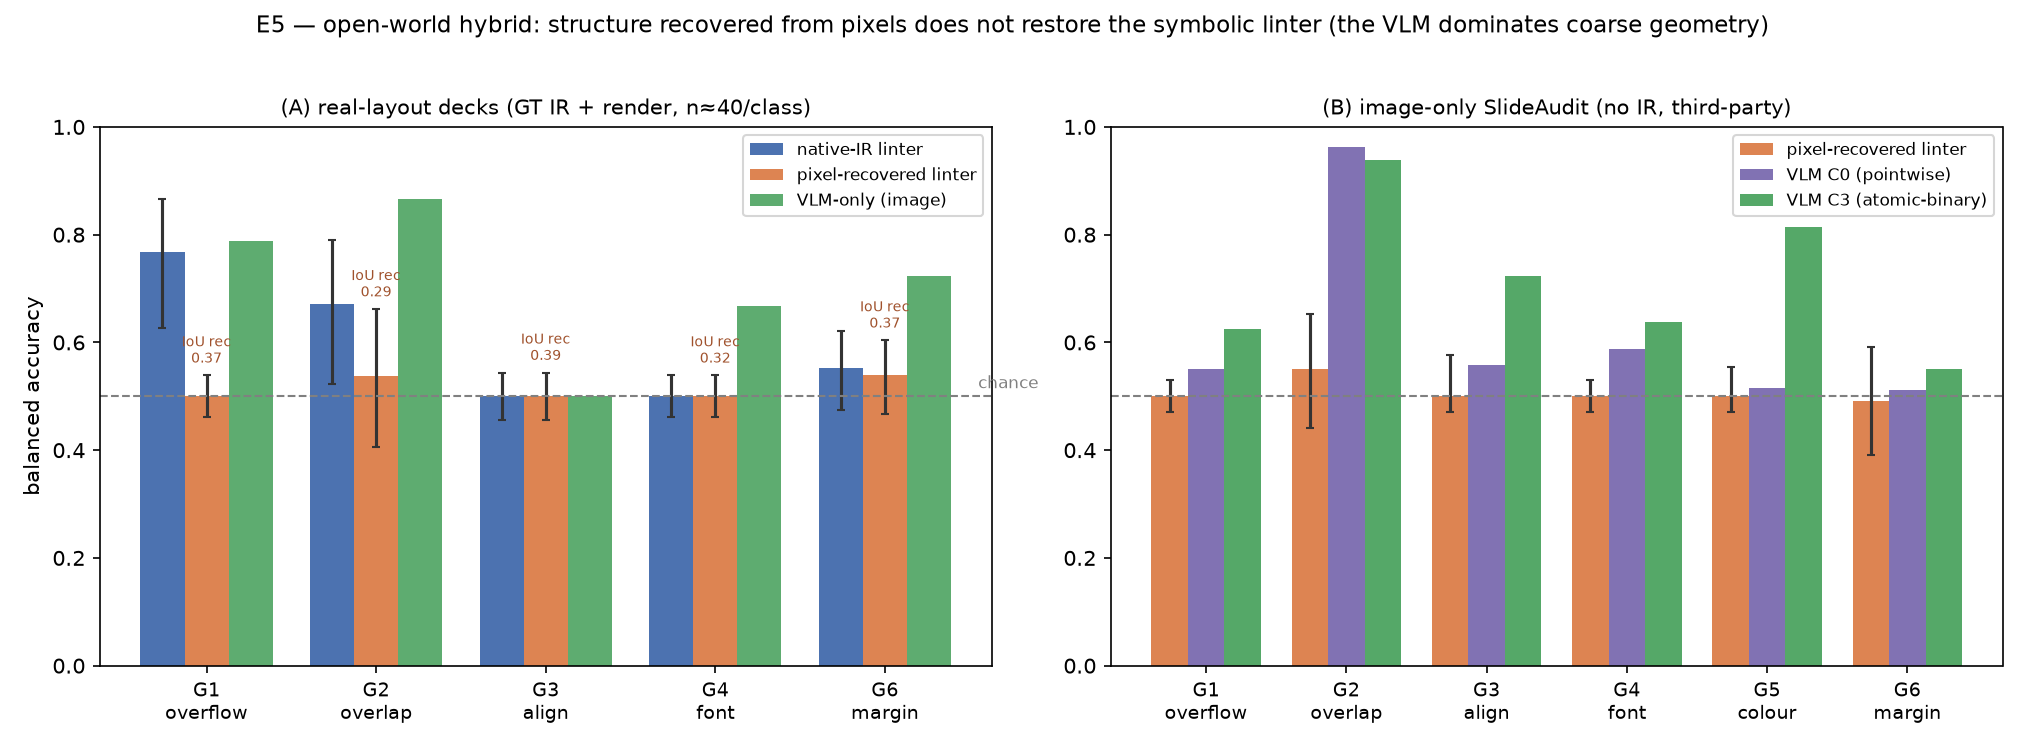
\includegraphics[width=\linewidth]{figs/fig8_open_world_recovery.png}
\caption{\textbf{Open-world hybrid: structure recovered from pixels does not restore the symbolic linter.}
A document-layout detector (PP-DocLayoutV2) recovers element boxes from the render; the \emph{same} geometry
linter runs on them. \textbf{(A)} real-layout decks (GT IR + render, $n{\approx}40$/class): native-IR linter vs.\
pixel-recovered linter vs.\ VLM-only floor, Wilson CIs; recovered structure rescues only overlap (\g{G2}) and is
silent on fine geometry, while the VLM dominates every class. \textbf{(B)} image-only \textsc{SlideAudit} (no IR,
third-party): the recovered linter clears chance only on \g{G2}; the C3-elicited VLM is far stronger. The linter's
near-zero-FP advantage requires clean native IR.}
\label{fig:openworld}
\end{figure}

% [E6 downstream-null] Per todo_0625 R4: the bounded/absent downstream effect is quarantined out of the body
% and scoped in Limitations (\S\ref{sec:limits}) in <=2 sentences (the axis-mismatch caution + the actionability
% A/B numbers are retained there). The full E6 paragraph and Fig.~9 (figs/fig9_unfloored_downstream.png) are cut
% from the body here, to be restored as an appendix figure at R11 if desired. Underlying data unchanged in repo.

% =====================================================================
\section{Limitations}\label{sec:limits}
% =====================================================================

We now report a human spot-check on the rebuilt corpus, but not an inter-annotator or deployment-time human
baseline. The paper's contribution is the \emph{diagnosis} (which bottleneck a defect hits) and the deterministic prescription
that follows from it; matching or exceeding human inspectors is a different claim we do not make. On the
rebuilt v2 sample, every sampled defect is judged visible and every clean twin clean (73/73; the auditable
structure-carrying subset is 55/55 source-faithful), so the paper's use of \g{G3}/\g{G5} rests on corrected
human-verified samples rather than the stale legacy framing.

Three scope bounds qualify the evidence. The real-layout attribution (\S\ref{sec:external}) uses \emph{injected}
defects (real geometry, renderer, and oracle, but not naturally-occurring), so the image-only,
naturally-defective \textsc{SlideAudit} set remains our complementary real probe. The reward audit covers five
published scorers and one closed judge; its document-reward miss is instance-level, and a second document/design
reward (PosterReward) and an InternLM-family reward (PloRA) were not stood up, so the categorical read rests on
the two general-multimodal backbones and the same-backbone CLIP-IQA/LAION dissociation. Last, the
examiner$\to$generation \emph{downstream} effect is near-null: examiner quality correlates $+0.66$ with
self-refine gain under a strong generator but at sub-1\% magnitude, and collapses to $0.00$ under an unfloored
weak generator ($1.43\times$ the headroom); a controlled A/B locates this as an axis mismatch, since the weak
generator's headroom is deck \emph{coverage}, which a layout critic does not move (quality change
$\Delta q{=}{+}0.00$ vs.\ a coverage critique's ${+}0.32$), so the examiner's evidence is its intrinsic and
case-study performance, not this loop.

Two caveats temper the central claims, both controlled in the body. First, the forced-choice and atomic-binary
elicitations supply a contrastive reference and a named target the pointwise format withholds; the C0+ and
guess-floor controls (\S\ref{sec:elicit}, Fig.~\ref{fig:decomp}) therefore scope strong format suppression to
\g{G7} and identify \g{G1}/\g{S6} as reference-assisted. Second, the 0.86 mean balanced accuracy and strict
6/9 coverage are \emph{native-structure} results: on image-only real decks the hybrid degrades to VLM-only,
and recovering structure from pixels does not close the gap (\S\ref{sec:external}, Fig.~\ref{fig:openworld}).
They are therefore an upper bound for IR-owning generation agents; on bare third-party pixels the deployable
critic is the C3-elicited VLM.

% =====================================================================
\section{Conclusion}
% =====================================================================

A slide-defect critic should not be one model. Telling apart sub-perceptual, format-suppressed, and
reference-assisted failures yields a deterministic method prescription: declared geometry to a symbolic
linter, targeted single-slide elicitation for format suppression, paired references where comparison resolves
the defect, and a semantic text/examiner module for page semantics. Compute-matched controls show that atomic
recovery is not purchased with extra inference. The prescribed composition reaches .957 on held-out validation;
a later frozen image-arm check scores .826 with unresolved reference requests counted as misses. \g{S6} clean false positives, failed pixel-recovered structure,
and the \textsc{SlideAudit} transfer gap delimit the result.

% =====================================================================
\appendix
\section{SlideAudit crosswalk}\label{app:slideaudit-crosswalk}
% =====================================================================

\begin{table}[t]
\centering
\footnotesize
\setlength{\tabcolsep}{3pt}
\caption{Crosswalk between our G/S classes and the 19-dimensional \textsc{SlideAudit} taxonomy. Empty entries are
intentional off-taxonomy semantic or deck-level defects; \g{G7} refines, rather than duplicates, SlideAudit's
content-overflow/cut-off category by adding the declared-legal-box criterion that makes the defect linter-blind.}
\label{tab:slideaudit-crosswalk}
\begin{tabular}{@{}p{0.22\linewidth}p{0.40\linewidth}p{0.29\linewidth}@{}}
\toprule
Our class & \textsc{SlideAudit} class & Relation \\
\midrule
\g{G1} text overflow & Content Overflow/Cut-off & equivalent \\
\g{G2} element overlap & Occluded Content & equivalent \\
\g{G3} alignment offset & Content Alignment Issues & equivalent \\
\g{G4} font-size inconsistency & Improper Font Sizing & equivalent \\
\g{G5} brand-color violation & Excessive or Inconsistent Color Usage; Inappropriate or Mismatched Color Combinations & equivalent \\
\g{G6} margin violation & Unbalanced Space Distribution & near-equivalent; safe-margin bleed is a special case \\
\g{G7} render-containment overflow & Content Overflow/Cut-off; related to Improper Image Sizing & our extension; same visual symptom plus declared-legal-box criterion \\
\g{S1} title/body mismatch & -- & off-taxonomy content semantics \\
\g{S2} narrative-order break & -- & off-taxonomy deck-level ordering \\
\g{S3} terminology inconsistency & -- & off-taxonomy cross-slide terminology \\
\g{S4} density violation & Excessive Text Volume & equivalent \\
\g{S5} missing logic section & -- & off-taxonomy deck-level completeness \\
\g{S6} image/text contradiction & Irrelevant Visual Content (nearest) & nearest only; contradiction rather than relevance \\
\bottomrule
\end{tabular}
\end{table}

% =====================================================================
\section*{Reproducibility}
% =====================================================================
\small
All analysis scripts, the defect injector, the two linters, the elicitation harness (including the C0+
coverage-vs-format control, \texttt{part3\_elicit.py --condition C0plus}), the deterministic hybrid critic, the
multi-reward audit adapters, the real-layout (\textsc{Zenodo10K}) IR/inject/render pipeline, and the per-Part
reports are released. A reproducibility bundle with paired manifests and per-item rollout CSVs is available
under \texttt{release/part3/} (generated by
\texttt{scripts/part3\_reproducibility\_release.py}). Experiments ran on 4$\times$RTX~3080 (20\,GB) with vLLM-served open VLMs
(Qwen3.5/3.6, Gemma4, InternVL3.5, Ovis2.5), a QLoRA-finetuned Qwen3-VL-8B, five published reward scorers,
and one DashScope Qwen3.7-Max VLM-judge probe
(DocReward-3B; Skywork-VL-Reward-7B and PickScore; a LAION aesthetic predictor and CLIP-IQA) behind a uniform
adapter; serving recipes
(tensor-parallel, AWQ, disabled thinking, fp8-KV caveats on Ampere) are in the repository. Weights, renders,
raw rollouts, and upstream licensed items are not redistributed; these omissions are licensing-constrained,
not convenience-constrained. Every balanced-accuracy cell in the tables and figures carries its 95\%
Wilson interval and per-cell $n$; the full family of paired tests is reported with Holm (FWER) and
Benjamini--Hochberg (FDR) multiplicity correction over all 85 reported significance tests (the original 61
plus the 24 compute-matched contrasts; released multiplicity report), and headline claims are stated as
surviving or downgraded under that correction.

% =====================================================================
\begin{thebibliography}{99}\small
% NOTE: arXiv titles/ids verified on 2026-06-22 (the 10 core ids via the arXiv API; skyworkvl 2505.07263 via
% web search across arxiv.org + the HF model card). laionaes has no arXiv paper -- it is a 2022 software artifact, cited as such.
% NOTE: 2026-06-24 (E7) re-verified the concurrent-2026 ids by web search w/ independent corroboration:
% rankscore 2604.25235 (github.com/divake/VLM-Judge-Uncertainty), aeslides 2604.22840 (github.com/ympan0508/aeslides, HF papers),
% reasoningbench 2512.21329 (arXiv html v2) -- all real concurrent work, not forward-fabricated. Added comparative 2307.07889
% (Liusie et al., EACL 2024 = 2024.eacl-long.8) and pairpoint 2504.14716 (Tripathi et al., OpenReview uyX5Vnow3U) for the
% relative-vs-absolute elicitation claim in Sec. Related Work.
\bibitem{chartbottleneck} Liu et al. On the Perception Bottleneck of VLMs for Chart Understanding. arXiv:2503.18435.
\bibitem{hiddeninplainsight} Fu, Bonnen, Guillory, Darrell. Hidden in Plain Sight: VLMs Overlook Their Visual Representations. arXiv:2506.08008.
\bibitem{mmvp} Tong et al. Eyes Wide Shut? Exploring the Visual Shortcomings of Multimodal LLMs. CVPR 2024; arXiv:2401.06209.
\bibitem{reasoningbench} Wang et al. Your Reasoning Benchmark May Not Test Reasoning: Revealing Perception Bottleneck in Abstract Reasoning Benchmarks. arXiv:2512.21329.
\bibitem{led} Heo, Hwang, Jung, Jung. LED Benchmark: Diagnosing Structural Layout Errors for Document Layout Analysis. arXiv:2507.23295.
\bibitem{rankscore} Kumar et al. VLM Judges Can Rank but Cannot Score: Task-Dependent Uncertainty in Multimodal Evaluation. arXiv:2604.25235.
\bibitem{comparative} Liusie, Manakul, Gales. LLM Comparative Assessment: Zero-shot NLG Evaluation through Pairwise Comparisons using Large Language Models. EACL 2024; arXiv:2307.07889.
\bibitem{pairpoint} Tripathi, Wadhwa, Durrett, Niekum. Pairwise or Pointwise? Evaluating Feedback Protocols for Bias in LLM-Based Evaluation. arXiv:2504.14716.
\bibitem{aeslides} Pan et al. AeSlides: Incentivizing Aesthetic Layout in LLM-Based Slide Generation via Verifiable Rewards. arXiv:2604.22840.
\bibitem{evopresent} Liu et al. Presenting a Paper is an Art: Self-Improvement Aesthetic Agents for Academic Presentations (EvoPresent/PresAesth). arXiv:2510.05571.
\bibitem{autopresent} Ge et al. AutoPresent: Designing Structured Visuals from Scratch. CVPR 2025; arXiv:2501.00912.
\bibitem{vlmslideeval} Kang, Bao, Goswami. VLM-SlideEval: Evaluating VLMs on Structured Comprehension and Perturbation Sensitivity in PPT. arXiv:2510.22045.
\bibitem{slideaudit} Zhang, Chen, Zhong, Wobbrock. SlideAudit: A Dataset and Taxonomy for Automated Evaluation of Presentation Slides. arXiv:2508.03630.
\bibitem{docreward} Liu et al. DocReward: A Document Reward Model for Structuring and Stylizing. arXiv:2510.11391.
\bibitem{skyworkvl} Wang et al. Skywork-VL Reward: An Effective Reward Model for Multimodal Understanding and Reasoning. arXiv:2505.07263; weights \texttt{Skywork/Skywork-VL-Reward-7B}.
\bibitem{laionaes} LAION-AI. Aesthetic Predictor: a linear estimator on CLIP for image aesthetic quality (LAION-Aesthetics). Software, 2022. \url{https://github.com/LAION-AI/aesthetic-predictor}.
\bibitem{pickscore} Kirstain et al. Pick-a-Pic: An Open Dataset of User Preferences for Text-to-Image Generation. NeurIPS 2023; arXiv:2305.01569; weights \texttt{yuvalkirstain/PickScore\_v1}.
\bibitem{clipiqa} Wang, Chan, Loy. Exploring CLIP for Assessing the Look and Feel of Images. AAAI 2023; arXiv:2207.12396.
\bibitem{zenodo10k} Zheng et al. PPTAgent: Generating and Evaluating Presentations Beyond Text-to-Slides (introduces the Zenodo10K corpus of real \texttt{.pptx}). arXiv:2501.03936; dataset \texttt{Forceless/Zenodo10K}.
\bibitem{doclaynet} Pfitzmann et al. DocLayNet: A Large Human-Annotated Dataset for Document-Layout Analysis. KDD 2022; arXiv:2206.01062.
\bibitem{publaynet} Zhong, Tang, Jimeno Yepes. PubLayNet: largest dataset ever for document layout analysis. ICDAR 2019; arXiv:1908.07836.
\end{thebibliography}

\end{document}
